\documentclass{article}
\usepackage[usenames,dvipsnames]{xcolor}
\usepackage{array}
\usepackage{float}
\usepackage{amsmath}
\usepackage{color}
\usepackage{graphicx}
\usepackage[utf8]{inputenc}
\usepackage[T1]{fontenc}
\usepackage[english]{babel}
\usepackage[makeroom]{cancel}

\definecolor{bg}{rgb}{0.95,0.95,0.95}

\begin{document}
\title{\textbf{''Introduction to Artificial Intelligence: Homework \#5''}}
\author{LAINE Bastien \#20156441}
\date{Nov. 18th 2015}
\maketitle
\tableofcontents

\newpage
    \section{Problem 1}
        \subsection{A}
        \subsection{B}
    \section{Problem 2}
        \subsection{A}
            We begin with the whole set of example.\\
            First, we compute the entropy of this step using the formula:
            \[
                \sum_{i\in\{0, 1\}} -p_i.\log_2(p_i)
            \]
            Then, we'll try to divide our set according to each input.\\
            Once done, we compute the average entropy of the 2 new set by ponderating both entropy by their Cardinality over the parent's cardinality.\\
            then, we choose the ``most interesting split'', that is to say the one whose entropy is maximum.\\

            Then, we compute again this step, but for our two new sub set. We'll stop our iteration when we found a leaf, that is to say a state where all of the ``outputs'' are the same (either 0 or 1 in our case)\\
            Since such a process is boring, I've developed a Bash script, whose goal is to create the graph. Executing it generate a PlantUML file. (Dependencie: bc)\\

            Finaly, the final result is the following:
            \begin{figure}[H]
                \centering
                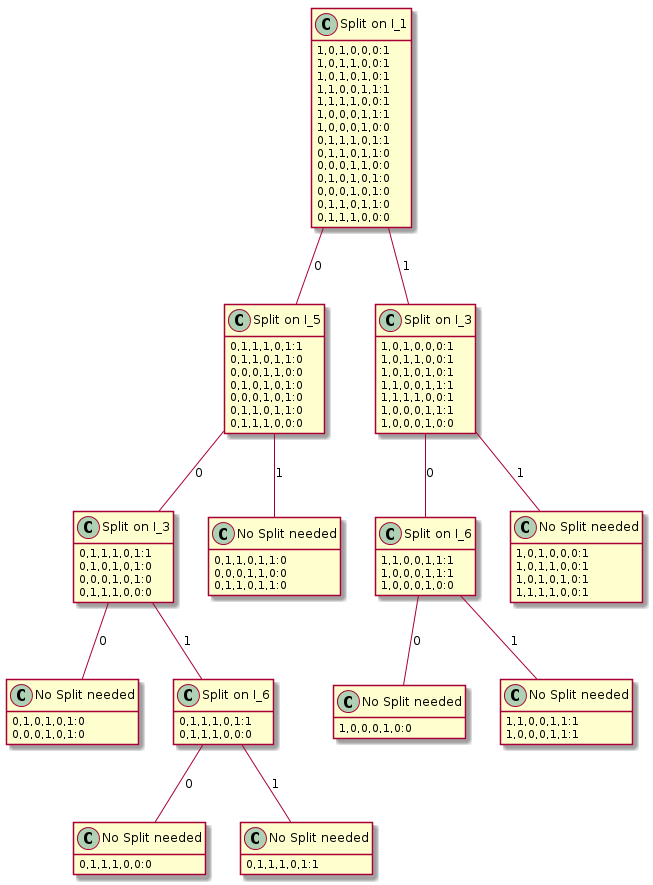
\includegraphics[scale=0.5]{problem2/graph.png}
                \caption{Final decision tree}
                \label{Final decision tree}
            \end{figure}


    \section{Problem 3}
        \subsection{A}
    \section{Problem 4}
        \subsection{A}
        \subsection{B}
        \subsection{C}
        \subsection{D}
            \begin{tabular}{|c|c|}
                \hline
                Interation & Error \\
                \hline
                40000 & \\
                \hline
                49000 & \\
                \hline
                $\cdots$ & \\
                \hline
                49000 & \\
                \hline
                Validation data & \\
                \hline
                Test data & \\
                \hline
            \end{tabular}
        \subsection{E}
\end{document}
